\section{大规模向量加法：内存限制与分块处理策略}

\subsection{引言：从中小规模到超大规模向量}

在之前的项目中，创建了 CUDA 程序来实现两个向量的加法，但那些向量的规模较小。本章将涵盖相同的应用程序——向量加法，但专注于尺寸大得多的向量。这个任务不会像之前的项目那样直截了当，将更加复杂。很可能会遇到几个挑战，本章将在遇到每一个挑战或问题时指出它，并提供相应的解决方案。

在上一个项目中，向量的大小是 2048 个元素，分配了两个线程块（block），每个块包含 1024 个线程。本章将把向量大小增加到超过 4 亿个元素。

当前的向量大小设定为 $1024 \times 432 \times 1024$，确实超过了 4 亿个元素。

转到启动核函数（Kernel）的指令。在这条指令中，使用每块 1024 个线程。为了处理所有这些元素，必须调整应用程序中的主要配置，即块数（Grid Size）和每块线程数（Block Size）。这代表了 GPU 的最大限制。对于网格大小（即块的数量），使用 $1024 \times 432$ 个块。这段代码中的其他所有内容都与之前的项目类似，不编辑其他部分。这两个配置的乘积应等于每个向量中的元素总数。

现在编译并运行。由于在处理很大的向量尺寸，这个应用程序的执行将花费一些时间。如所示，一切正常，结果显示如图。可以在这里选择任意一行，测试 $A + B$ 是否等于 $C$ 的值。无论是编译还是运行应用程序，都没有出现编译错误或运行时错误。

\subsection{挑战一：超出主机内存限制}

进一步增加向量尺寸时，问题出现了。到向量大小定义处复查一下，将 432 替换为 1024。现在每个向量都有超过 10 亿个元素。编译后发现没有任何编译错误。运行应用程序，如图所示，代码未能正确运行。代码中用于验证结果的 for 循环输出没有再显示在终端上。此外，可以注意到，如果错误码为零，则表示没有错误；如果是非零数字，则表示遇到了运行时错误。该应用程序中没有编译错误。

需要思考一下这个问题：为什么在这个应用程序中遇到了错误？可能的原因是什么？


\begin{figure}
    \centering
    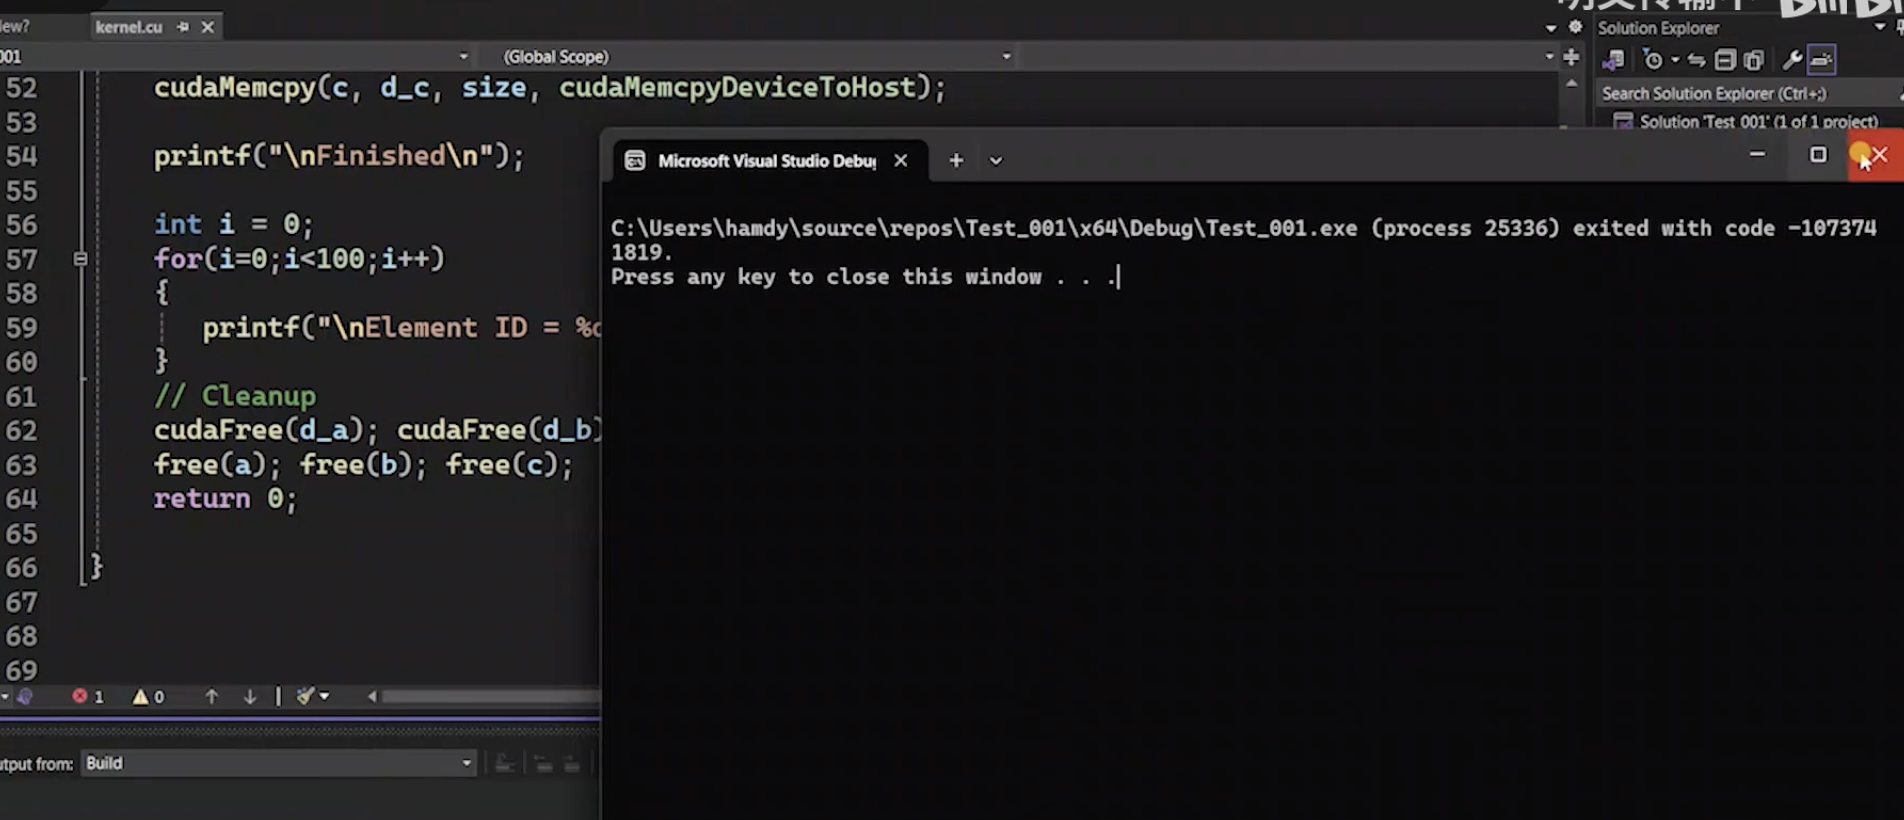
\includegraphics[width=0.75\linewidth]{resources/cuda-080.png}
    \caption{}
    \label{fig:placeholder}
\end{figure}


\subsection{调试策略：使用 printf 定位问题}

下面提供解决方案。有很多调试策略可以找到确切的问题所在。在这种情况下，最有效的调试技巧之一是使用 \texttt{printf} 函数。在应用程序的不同位置放置许多 \texttt{printf} 指令，然后运行应用程序，利用终端上的输出来定位有问题的代码行。

例如，在开头写第一个 \texttt{printf("hello 00\textbackslash n");}，然后将这条指令复制到不同的位置，并依次标记为 01、02 等。为什么需要在不同的位置放置 \texttt{printf} 指令？因为需要识别错误发生的具体位置。这与语法错误不同——如果移除一个分号，编译器会明确告知问题所在。但在当前情况下，遇到的是运行时错误而非编译错误。

编译成功后，看到终端打印了 "hello 00" 和 "hello 01"，但 "hello 02" 没有打印。这意味着错误发生在 "hello 01" 之后、"hello 02" 之前。结合上下文，发现 GPU 内存分配（\texttt{cudaMalloc}）本身没有报错，问题出在 CPU 端的主机内存分配上。

\subsection{根本原因分析}

为了理解这一点，查看 RAM（主机内存）中的可用空间。假设计算机总共有 16 GB RAM，当前已使用约 10 GB，剩余约 6 GB 可用空间。回到代码，当运行应用程序时，流程是为向量 A 分配空间并初始化，然后为 B 分配并初始化，最后为 C 分配空间。

当向量维度设置为 $1024 \times 1024 \times 1024$ 时，单个向量的元素数量为 $1,073,741,824$。由于每个整数元素占 4 字节，单个向量的大小为：
\[\frac{1024 \times 1024 \times 1024 \times 4 \text{Bytes}}{1024^3} = 4 \text{ GB}\]要存储三个向量（A、B、C），总共需要 12 GB 主机内存，而计算机上没有这么多可用空间。这就是导致运行时失败的根本原因。虽然 GPU 显存可能足够，但 \texttt{malloc} 在主机端分配内存时失败了。

\subsection{解决方案：数据分块（Chunking）处理}

解决此问题的方案是将每个向量分成小块（chunks）。具体使用多少块取决于可用内存。假设有 4 至 5 GB 可用空间，每个数据块的大小应小于此限制。

例如，将维度中的 1024 替换为 128。这意味着将把每个向量分成 8 块，因为 $1024 / 128 = 8$。使用这个"块大小"（chunk size）来分割向量。处理流程如下：取 A 的第一块和 B 的第一块相加，将结果存入 C 的第一块；完成后释放这些临时缓冲区占用的内存；然后转到向量的第二部分，依此类推，直到处理完所有部分。

\subsection{分块代码实现逻辑}

以下是修改后的核心逻辑说明：

\begin{enumerate}
    \item \textbf{参数定义}：定义总大小（total size）、数据块大小（chunk size）以及块数量（num chunks = total size / chunk size）。线程块大小仍保持为每块 1024 个线程。
    \item \textbf{核函数}：GPU 核函数和初始化函数无需修改，仅需传入数据块指针而非完整向量指针。
    \item \textbf{内存分配}：不再为整个向量分配空间，而是仅为当前数据块分配空间。使用 \texttt{malloc(chunk\_size * sizeof(int))} 为 \texttt{chunk\_A}、\texttt{chunk\_B}、\texttt{chunk\_C} 分配主机内存。GPU 端同样只分配数据块大小的显存。
    \item \textbf{迭代处理}：使用 for 循环遍历所有数据块。在每次迭代中：
    \begin{itemize}
        \item 计算当前偏移量（offset = i * chunk\_size）；
        \item 初始化或加载当前块的 A 和 B 数据；
        \item 使用 \texttt{cudaMemcpy} 将数据块拷贝到 GPU；
        \item 执行核函数进行向量加法；
        \item 使用 \texttt{cudaMemcpy} 将结果从 GPU 拷回主机的 \texttt{chunk\_C}；
        \item 验证或输出当前块的结果；
        \item 释放当前块的主机和设备内存，为下一次迭代做准备。
    \end{itemize}
\end{enumerate}

\subsection{验证与结果}

编译并运行修改后的代码。编译成功。运行时，终端打印了每个数据块的偏移量：0、128、256……直到第 8 个块。这证实了循环正确执行了 8 次迭代。

观察内存使用情况，仅使用了约 1 GB 左右的额外空间，因为只为两个数据块（A 和 B 的当前块）分配了空间，而不是三个完整的向量。当程序完成并释放内存后，可用空间恢复到了初始水平。

最终结果是正确的，例如 $13 + 77 = 90$ 等验证均通过。这就是本章讨论的第一个挑战及其完整的解决方案：通过数据分块技术突破主机内存限制，实现超大规模向量运算。

